%!Tex Root = ../Tutorat7.tex
% ./Packete.tex
% ./Design.tex
% ./Deklarationen.tex
% ./Aufgabe2.tex
% ./Aufgabe3.tex
% ./Aufgabe4.tex
% ./Bonus.tex

\section{Task 1}

\setcounter{task}{1}

\begin{frame}[allowframebreaks]{Task 1}{Scheduling with Pipeline Resources}
  \begin{tasknoinc}
    \begin{columns}
      \begin{column}{.3\textwidth}
        \centering
        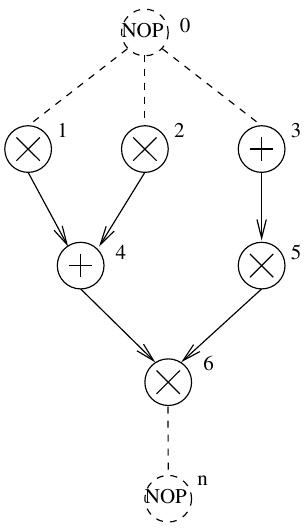
\includegraphics[width=.7\textwidth]{./figures/task1_pipeline_resource_sequence_graph.png}
      \end{column}
      \begin{column}{.7\textwidth}
        \centering
        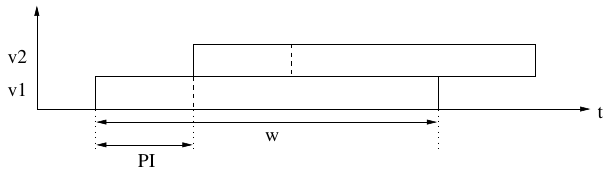
\includegraphics[width=.7\textwidth]{./figures/task1_tasks_on_pipeline_resource.png}
      \end{column}
    \end{columns}
  \end{tasknoinc}
\end{frame}
\begin{frame}[fragile]{Task 1}{Scheduling with Pipeline Resources}
  \begin{solutionnoinc}
    \centering
    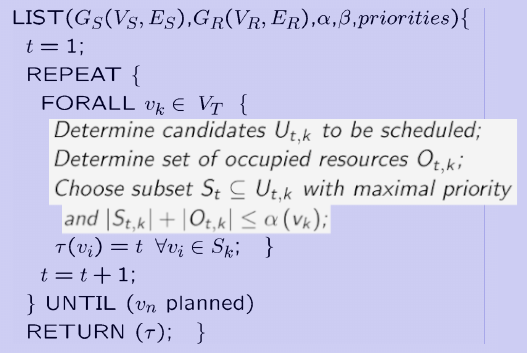
\includegraphics[width=0.6\textwidth]{./figures/list_scheduling.png}
  \end{solutionnoinc}
\end{frame}
\begin{frame}[fragile]{Task 1}{Scheduling with Pipeline Resources}
  \begin{solution}
      % \begin{algorithm}[H]
      % [...]\;
      % Determine candidates $U_{t, k}$ to be scheduled\;
      % Determine set of occupied resources $O_{t, k}$\;
      % Choose subset $S_t \subseteq U_{t, k}$ with maximal priority and $\left|S_{t, k}\right|+\left|O_{t, k}\right| \leq \alpha\left(v_k\right)$\;
      % [...]\;
      % \end{algorithm}
    \begin{itemize}
      \item $O_{t, k}$ is the set of resources of type $k$ that are occupied in the time slot $t$ and are not yet available for the following operation. On each of these resources exactly one operation is executed in a pipeline-interval.
      \item $O_{t, k} = \left\{v_s: \beta\left(v_s\right)=v_t \wedge \tau\left(v_s\right)<t<\tau\left(v_s\right)+PI\right\}$ instead of $T_{t, k} = \left\{v_s: \beta\left(v_s\right)=v_t \wedge \tau\left(v_s\right)<t<\tau\left(v_s\right)+w\left(v_s, v_t\right)\right\}$
    \end{itemize}
  \end{solution}
\end{frame}

\begin{frame}{Task 1}{Scheduling with Pipeline Resources}
  \begin{solutionnoinc}
    \begin{itemize}
      \item \alert{without pipelining}:
    \end{itemize}
      \centering
      \fontsize{3}{4}\selectfont
      \begin{tabular}{c|c|l|l|l|}
      \hline$t$                  & $k$   & $U_{t, k}$ & $T_{t, k}$ & $S_{t, k}$ \\
      \hline \multirow{2}{*}{0}  & $r_1$ & v3         & -          & v3 \\
      \cline { 2 - 5 }           & $r_2$ & v1 v2      & -          & v1 \\
      % ------------------------------------------------------------------
      \hline \multirow{2}{*}{1}  & $r_1$ & -          & v3         & -  \\
      \cline { 2 - 5 }           & $r_2$ & v2         & v1         & -  \\
      % ------------------------------------------------------------------
      \hline \multirow{2}{*}{2}  & $r_1$ & -          & -          & -  \\
      \cline { 2 - 5 }           & $r_2$ & v2 v5      & v1         & -  \\
      % ------------------------------------------------------------------
      \hline \multirow{2}{*}{3}  & $r_1$ & -          & -          & -  \\
      \cline { 2 - 5 }           & $r_2$ & v2 v5      & v1         & -  \\
      % ------------------------------------------------------------------
      \hline \multirow{2}{*}{4}  & $r_1$ & -          & -          & -  \\
      \cline { 2 - 5 }           & $r_2$ & v5         & -          & v2 \\
      % ------------------------------------------------------------------
      \hline \multirow{2}{*}{5}  & $r_1$ & -          & -          & -  \\
      \cline { 2 - 5 }           & $r_2$ & v5         & v2         & -  \\
      % ------------------------------------------------------------------
      \hline \multirow{2}{*}{6}  & $r_1$ & -          & -          & -  \\
      \cline { 2 - 5 }           & $r_2$ & v5         & v2         & -  \\
      % ------------------------------------------------------------------
      \hline \multirow{2}{*}{7}  & $r_1$ & -          & -          & -  \\
      \cline { 2 - 5 }           & $r_2$ & v5         & v2         & -  \\
      % ------------------------------------------------------------------
      \hline \multirow{2}{*}{8}  & $r_1$ & v4         & -          & v4 \\
      \cline { 2 - 5 }           & $r_2$ & v5         & -          & v5 \\
      % ------------------------------------------------------------------
      \hline \multirow{2}{*}{9}  & $r_1$ & -          & v4         & -  \\
      \cline { 2 - 5 }           & $r_2$ & -          & v5         & -  \\
      % ------------------------------------------------------------------
      \hline \multirow{2}{*}{10} & $r_1$ & -          & -          & -  \\
      \cline { 2 - 5 }           & $r_2$ & -          & v5         & -  \\
      % ------------------------------------------------------------------
      \hline \multirow{2}{*}{11} & $r_1$ & -          & -          & -  \\
      \cline { 2 - 5 }           & $r_2$ & -          & v5         & -  \\
      % ------------------------------------------------------------------
      \hline \multirow{2}{*}{12} & $r_1$ & -          & -          & -  \\
      \cline { 2 - 5 }           & $r_2$ & v6         & -          & v6 \\
      % ------------------------------------------------------------------
      \hline \multirow{2}{*}{13} & $r_1$ & -          & -          & -  \\
      \cline { 2 - 5 }           & $r_2$ & -          & v6         & -  \\
      % ------------------------------------------------------------------
      \hline \multirow{2}{*}{14} & $r_1$ & -          & -          & -  \\
      \cline { 2 - 5 }           & $r_2$ & -          & v6         & -  \\
      % ------------------------------------------------------------------
      \hline \multirow{2}{*}{15} & $r_1$ & -          & -          & -  \\
      \cline { 2 - 5 }           & $r_2$ & -          & v6         & -  \\
      % ------------------------------------------------------------------
      \hline \multirow{2}{*}{15} & $r_1$ & -          & -          & -  \\
      \cline { 2 - 5 }           & $r_2$ & -          & -          & -  \\
      \hline
      \end{tabular}
  \end{solutionnoinc}
\end{frame}
\begin{frame}{Task 1}{Scheduling with Pipeline Resources}
  \begin{solutionnoinc}
      \centering
      \fontsize{4}{5}\selectfont
      \begin{tabular}{c|c|l|l|l|}
      \hline$t$ & $k$ & $U_{t, k}$ & $O_{t, k}$ & $S_{t, k}$ \\
      \hline \multirow{2}{*}{0} & $r_1$ & & & \\
      \cline { 2 - 5 } & $r_2$ & & & \\
      \hline \multirow{2}{*}{1} & $r_1$ & & & \\
      \cline { 2 - 5 } & $r_2$ & & & \\
      \hline \multirow{2}{*}{2} & $r_1$ & & & \\
      \cline { 2 - 5 } & $r_2$ & & & \\
      \hline \multirow{2}{*}{3} & $r_1$ & & & \\
      \cline { 2 - 5 } & $r_2$ & & & \\
      \hline \multirow{2}{*}{4} & $r_1$ & & & \\
      \cline { 2 - 5 } & $r_2$ & & & \\
      \hline \multirow{2}{*}{5} & $r_1$ & & & \\
      \cline { 2 - 5 } & $r_2$ & & & \\
      \hline \multirow{2}{*}{6} & $r_1$ & & & \\
      \cline { 2 - 5 } & $r_2$ & & & \\
      \hline \multirow{2}{*}{7} & $r_1$ & & & \\
      \cline { 2 - 5 } & $r_2$ & & & \\
      \hline \multirow{2}{*}{8} & $r_1$ & & & \\
      \cline { 2 - 5 } & $r_2$ & & & \\
      \hline \multirow{2}{*}{9} & $r_1$ & & & \\
      \cline { 2 - 5 } & $r_2$ & & & \\
      \hline \multirow{2}{*}{10} & $r_1$ & & & \\
      \cline { 2 - 5 } & $r_2$ & & & \\
      \hline \multirow{2}{*}{11} & $r_1$ & & & \\
      \cline { 2 - 5 } & $r_2$ & & & \\
      \hline \multirow{2}{*}{12} & $r_1$ & & & \\
      \cline { 2 - 5 } & $r_2$ & & & \\
      \hline
      \end{tabular}
  \end{solutionnoinc}
\end{frame}
\begin{frame}{Task 1}{Scheduling with Pipeline Resources}
  \begin{solutionnoinc}
      \centering
      \fontsize{4}{5}\selectfont
      \begin{tabular}{c|c|l|l|l|}
      \hline$t$                  & $k$   & $U_{t, k}$ & $O_{t, k}$ & $S_{t, k}$ \\
      \hline \multirow{2}{*}{0}  & $r_1$ & $v_3$      & $-$        & $v_3$      \\
      \cline { 2 - 5 }           & $r_2$ & $v_1, v_2$ & $-$        & $v_1$      \\
      \hline \multirow{2}{*}{1}  & $r_1$ & $-$        & $v_3$      & $-$        \\
      \cline { 2 - 5 }           & $r_2$ & $v_2$      & $v_1$      & $-$        \\
      \hline \multirow{2}{*}{2}  & $r_1$ & $-$        & $-$        & $-$        \\
      \cline { 2 - 5 }           & $r_2$ & $v_2, v_5$ & $-$        & $v_2$      \\
      \hline \multirow{2}{*}{3}  & $r_1$ & $-$        & $-$        & $-$        \\
      \cline { 2 - 5 }           & $r_2$ & $v_5$      & $v_2$      & $-$        \\
      \hline \multirow{2}{*}{4}  & $r_1$ & $-$        & $-$        & $-$        \\
      \cline { 2 - 5 }           & $r_2$ & $v_5$      & $-$        & $v_5$      \\
      \hline \multirow{2}{*}{5}  & $r_1$ & $-$        & $-$        & $-$        \\
      \cline { 2 - 5 }           & $r_2$ & $-$        & $v_5$      & $-$        \\
      \hline \multirow{2}{*}{6}  & $r_1$ & $v_4$      & $-$        & $v_4$      \\
      \cline { 2 - 5 }           & $r_2$ & $-$        & $-$        & $-$        \\
      \hline \multirow{2}{*}{7}  & $r_1$ & $-$        & $v_4$      & $-$        \\
      \cline { 2 - 5 }           & $r_2$ & $-$        & $-$        & $-$        \\
      \hline \multirow{2}{*}{8}  & $r_1$ & $-$        & $-$        & $-$        \\
      \cline { 2 - 5 }           & $r_2$ & $v_6$      & $-$        & $v_6$      \\
      \hline \multirow{2}{*}{9}  & $r_1$ & $-$        & $-$        & $-$        \\
      \cline { 2 - 5 }           & $r_2$ & $-$        & $v_6$      & $-$        \\
      \hline \multirow{2}{*}{10} & $r_1$ & $-$        & $-$        & $-$        \\
      \cline { 2 - 5 }           & $r_2$ & $-$        & $-$        & $-$        \\
      \hline \multirow{2}{*}{11} & $r_1$ & $-$        & $-$        & $-$        \\
      \cline { 2 - 5 }           & $r_2$ & $-$        & $-$        & $-$        \\
      \hline \multirow{2}{*}{12} & $r_1$ & $-$        & $-$        & $-$        \\
      \cline { 2 - 5 }           & $r_2$ & $-$        & $-$        & $-$        \\
      \hline
      \end{tabular}
  \end{solutionnoinc}
\end{frame}
\begin{frame}
  \begin{solutionnoinc}
    \begin{itemize}
      \item the resulting latency is $12$
    \end{itemize}
  \end{solutionnoinc}
\end{frame}
